\chapter{Marco Teórico}

Para automatizar el flujo operativo de recepción, clasificación y seguimiento en la Defensoría de Derechos Politécnicos (DDP), se implementará un clasificador de texto encargado de determinar la competencia o improcedencia de cada queja. El desarrollo de este motor se basará en modelos de aprendizaje supervisado, específicamente la Máquina de Soporte Vectorial (SVM) y Naive Bayes, este último como enfoque probabilístico fundamental.

\section{Problema de clasificación en el contexto de la DDP}

Actualmente, la determinación de la competencia de una queja en la Defensoría de Derechos Politécnicos recae exclusivamente en el factor humano. Este proceso es llevado a cabo por abogados especialistas quienes, fundamentados en el Artículo 13 del Acuerdo de Creación y parámetros institucionales, analizan cada narrativa para decidir si el asunto entra en el ámbito de facultades de la Defensoría.

El conflicto no reside en la capacidad de los abogados para clasificar, sino en la carga operativa y la variabilidad del criterio manual. Al depender de una interpretación subjetiva de textos no estructurados, el flujo de recepción se vuelve lento y propenso a cuellos de botella. Por ello, surge la necesidad de un sistema de clasificación automatizado que actúe como un filtro inteligente, emulando la lógica jurídica para agilizar la respuesta institucional.

\subsection{Taxonomía de denuncias}
Para transformar este proceso manual en un modelo de aprendizaje automático, es necesario estructurar la taxonomía de las denuncias. Aunque el sistema final arroja un veredicto de naturaleza binaria (Competente o No Competente), la decisión depende de un análisis multidimensional basado en los siguientes criterios:

\begin{enumerate}
    \item \textbf{Identificación del Sujeto (Legitimación):} Se verifica que el quejoso sea un miembro de la comunidad politécnica (alumno con número de cuenta o empleado con número de trabajador) y que la autoridad señalada pertenezca a una unidad académica o administrativa del IPN.
    \item \textbf{Temporalidad (Plazo de 90 días):} La queja debe interponerse dentro de los noventa días siguientes a los hechos que la motivan. Si excede este tiempo, se clasifica automáticamente como improcedente.
    \item \textbf{Naturaleza del Conflicto (Exclusiones):} La competencia se descarta si el hecho es de carácter anónimo o si versa sobre materias ajenas a la Defensoría, específicamente:
    \begin{itemize}
        \item[3.1.] \textbf{Asuntos Laborales:} Conflictos obrero-patronales o sindicales que no entran en la esfera de derechos politécnicos.
        \item[3.2.] \textbf{Evaluaciones Académicas:} Inconformidades puramente sobre criterios de calificación, a menos que impliquen una vulneración de derechos humanos o politécnicos.
        \item[3.3.] \textbf{Resoluciones de otras instancias:} Casos que ya estén siendo atendidos o hayan sido resueltos por el Órgano Interno de Control o el Abogado General.
    \end{itemize}
    \item \textbf{Formalidad del Acto:} Se requiere que la queja contenga la descripción detallada de los actos, la firma o huella del promovente y, en caso de menores de edad, la validación del tutor.
    \item \textbf{Análisis de Reincidencia:} Aunque la queja sea nueva, el factor humano evalúa si el "afectador" (autoridad o docente) presenta un patrón de conducta registrado en otros expedientes del sistema, lo que ayuda a catalogar la gravedad y urgencia del asunto.
\end{enumerate}

\subsection{Clasificación multiclase vs multietiqueta}

Si bien el diseño de una arquitectura híbrida representa la solución óptima, para este sistema se ha optado por un enfoque de clasificación multiclase (binaria). Esta decisión se fundamenta en la viabilidad técnica: la implementación de una clasificación multietiqueta requeriría un volumen de datos de entrenamiento con el que no se cuenta actualmente. En contraste, el enfoque binario permite concentrar la muestra en solo dos categorías, garantizando una mayor densidad de datos por clase y, por ende, una mayor robustez en el entrenamiento del modelo.

\begin{itemize}
    \item Acorde al articulo 13, una queja no puede ser simultáneamente “Competente” e “Improcedente”.
    \item El sistema debe arrojar un veredicto definitivo para procesar el folio, o se admite o se rechaza.
    \item Dado que la competencia se define por la ausencia de improcedencia, el modelo debe asignar la queja a una sola categoría.
\end{itemize}

Una vez declarada la queja como competente, el sistema se beneficia de un enfoque multietiqueta para el análisis de los hechos:
\begin{itemize}
    \item Un solo relato de hechos puede contener múltiples vulneraciones. Por ejemplo, una queja puede catalogarse simultáneamente como "Violencia de Género", "Abuso de Autoridad" y "Afectación Académica".
    \item El uso de etiquetas múltiples permite al sistema detectar patrones más complejos. Si un docente tiene etiquetas recurrentes de "Acoso verbal" en diferentes expedientes, el sistema alerta sobre un escalamiento de violencia.
    \item Permite a los abogados filtrar casos por materias específicas para aplicar los mismos criterios de lógica y legalidad en la valoración de pruebas similares.
\end{itemize}

La transición de un modelo de decisión basado en el juicio humano hacia un sistema automatizado requiere de una infraestructura de datos robusta. No basta con definir los criterios legales de competencia; es imperativo establecer un flujo técnico que transforme la narrativa subjetiva del quejoso en una entrada estructurada que los algoritmos puedan procesar. A continuación, se detalla el ciclo de vida de los datos, el cual actúa como el puente operativo entre el Artículo 13 del Reglamento y la implementación de los modelos SVM y Naive Bayes.

\subsection{Ciclo de vida de los datos en el aprendizaje supervisado}

El ciclo de vida de los datos en este proyecto no es solo un proceso técnico, sino que debe alinearse estrictamente con los lineamientos del Artículo 13 del Reglamento de la Defensoría. Este ciclo garantiza que la información sea útil para entrenar los modelos de SVM y Naive Bayes mencionados anteriormente:

\begin{enumerate}
    \item \textbf{Captura de datos:} Los datos se originan cuando el quejoso interactúa con el sistema digital. Para cumplir con la Fracción II del Artículo 13, el sistema captura de forma estructurada el nombre, número de cuenta/empleado, la autoridad imputada y la descripción detallada de los hechos.
    \item \textbf{Procesamiento y Filtrado:}La descripción de los actos se somete a técnicas de Procesamiento de Lenguaje Natural (PLN) para identificar palabras clave relacionadas con las exclusiones de competencia (ej. "sindicato", "evaluación", "laboral").
    \item \textbf{Etiquetado (Supervisión):} Dado que es un aprendizaje supervisado, el modelo se entrena con el histórico de decisiones de los abogados. Cada expediente histórico se etiqueta como "Competente" (Admitida) o "No Competente" (Rechazo fundado y motivado) basándose en si cumplió con los lineamientos del Artículo 13.
    \item \textbf{División de Dataset:} Debido a la escasez de datos para etiquetas múltiples, se utiliza el conjunto de datos para fortalecer la clasificación binaria. Se divide la muestra en datos de entrenamiento (para que el modelo aprenda la correlación entre hechos y competencia) y datos de validación (para asegurar que el modelo pueda predecir correctamente la competencia de quejas nuevas).
    \item \textbf{Retroalimentación:} El modelo sugiere una clasificación al abogado. Si el factor humano corrige la sugerencia del sistema (por ejemplo, admitiendo una queja que el modelo sugirió rechazar), este dato se reincorpora al ciclo para re-entrenar el modelo y mejorar su precisión futura.
    \item \textbf{Anonimización y Resguardo:} Los datos permanecen activos para la detección de patrones de reincidencia. Al cumplirse el límite de 5 años de resguardo físico, la información digital puede permanecer anonimizada para fines estadísticos y de mejora continua del motor de clasificación.
\end{enumerate}


\section{Fundamentos lógicos}

\subsection{Inferencia Bayesiana (probabilidad a priori y a posteriori)}

La inferencia bayesiana es un método estadístico el cual permite actualizar la probabilidad de un evento a medida que se obtiene nueva evidencia o información, sigue siendo el Teorema de Bayes, indica cuál es la probabilidad de que desarrolle un determinado escenario, teniendo en cuenta un mínimo de dos alternativas, pues tienen que existir opciones en las que elegir, la formula prioriza tres conceptos:

\begin{enumerate}
    \item \textbf{Priorización y posterización:} En primer lugar, se utiliza una probabilidad previa que se actualizara a través de dato, de esta manera obtenemos probabilidad posterior, pues la idea es comprobar ese contraste.
    \item \textbf{Verosimilitud:} Representa la probabilidad de observar los términos específicos en la queja ($D$) asumiendo que esta pertenece a una categoría determinada ($H$). Permite medir qué tan bien los datos observados respaldan la clasificación sugerida. Si los datos no son verosímiles, se tendrán que consultar los sistemas de capacitación de estos.
    \item \textbf{Actuación iterativa:} Cuando más información se tenga, las probabilidades posteriores pueden ser previas.
\end{enumerate}

Probabilidad a priori es la probabilidad que se asigna a un evento antes de observar cualquier evidencia o realizar un experimento. Representa el conocimiento inicial o creencia sobre la posibilidad de un suceso, que puede basarse en información subjetiva, objetiva o una mezcla de ambas.

Probabilidad a posteriori es la probabilidad de un evento después de haber observado evidencia o realizado un experimento. Se calcula utilizando el Teorema de Bayes, que actualiza la probabilidad a priori con nueva información. Por ejemplo, si se sabe que una persona dio positivo en una prueba de enfermedad, la probabilidad a posteriori de que realmente tenga la enfermedad se calcula considerando la precisión de la prueba y la prevalencia de la enfermedad en la población.

La relación se expresa mediante el Teorema de Bayes:
\begin{equation}
P(H|D) = \frac{P(D|H) \cdot P(H)}{P(D)}
\end{equation}

En este caso, debemos decir que $P(H|D)$ es el resultado final de la probabilidad posterior de la hipótesis $H$ a partir de la evidencia $D$. Por otra parte, $P(D|H)$ es la verosimilitud; $P(H)$ la probabilidad previa y $P(D)$ la probabilidad posterior.

Esta fórmula se puede incluir en numerosos elementos y, también, cuando se diseñan modelos. Por eso este teorema, cuyo origen está en 1763, sigue teniendo especial importancia en las nuevas tecnologías.

\subsection{Algebra lineal en PLN}

Para que el modelo pueda aplicar los principios probabilísticos de Bayes, primero debe ser capaz de 'leer' el texto de forma matemática. El Álgebra Lineal proporciona la estructura necesaria para transformar las narrativas jurídicas en vectores numéricos, permitiendo que el motor de clasificación realice operaciones geométricas en un espacio de características de alta dimensionalidad.

Este modelo posibilita determinar la importancia de un termino en un documento especifico y entiende que los documentos pueden expresarse en función de estos vectores que recogen la frecuencia en que aparecen los términos en los documentos. Los términos que formaran esta matriz serán términos no vacíos, esto significa que contienen significado para el momento de recuperar información, teniéndolos almacenados en formato stemmed (reducidos los términos a una raíz común).

Este procedimiento se puede dividir en tres etapas:

\begin{enumerate}
    \item La primera es la \textbf{etapa de indexación de documentos} donde los términos que contienen información se extraen del texto de documento. Muchas de las palabras no describen el contenido, como los artículos y preposiciones, las palabras no significativas se eliminan del vector del documento, de esta manera, el documento solo se representará por palabras que contengan contenido representativo. Esta indexación puede basarse en la frecuencia de los términos, donde los términos tienen tanto alta como baja frecuencia dentro de un documento se consideran palabras funcionales. Para lograr hacer esta etapa de manera funcional, se hace uso de una lista de palabras comunes que se usan de manera frecuente, para así eliminar estas palabras que provocarían errores (stopwords), normalmente, el 40-50\% del numero total de palabras se elimina con ayuda de la lista de detención.
    \item La segunda etapa es la \textbf{ponderación de los términos} para mejorar la recuperación de documentos relevantes para el usuario, esta ponderación temporal se explica mediante la relación con el recuerdo y la especificidad con la precisión, este termino (ponderación) se basa completamente en estadísticas de un solo termino. Hay tres factores para la ponderación del término: factor de término, factor de frecuencia de recopilación y factor de normalización de longitud.
    \item La última etapa \textbf{clasifica el documento} con respecto a la consulta según una medida de similitud, esta se determina mediante el uso de coeficientes asociativos basados en el producto interno del vector de documento y el vector de consulta. La medida de similitud es el coeficiente del coseno, que mide el ángulo entre un vector de documento y el vector de consulta.
\end{enumerate}

\subsubsection{Espacios de características (N-dimensiones)}

Un espacio de características es una construcción matemática donde cada palabra única (después del proceso de stemming y eliminación de stopwords) se convierte en un eje o dimensión independiente.

Definimos las dimensiones si el vocabulario total de todas las quejas históricas de la DDP contiene $V$ términos únicos, entonces, cada queja se representa con un vector $x$ en un espacio de dimensiones $V$, denotado como $\mathbb{R}^V$.

Entonces, una queja especifica se define como:
\begin{equation}
\vec{x} = (w_1, w_2, w_3, \dots, w_V)
\end{equation}

Donde $w_i$ representa el peso del termino $i$ en esa queja. Si una palabra $x$ tiene un peso alto en el vector, este apuntara hacia un región del espacio asociada históricamente  a la improcedencia. Dado que el lenguaje es vasto, el espacio de características suele ser de alta dimensionalidad, lo que significa que la mayoría de los componentes del vector serán cero, ya que una sola queja no contiene todas las palabras.

\subsubsection{Métricas de proximidad}

Una vez que las quejas están proyectadas en el espacio de características, el motor de clasificación deberá medir que tan cerca esta una queja nueva de los ejemplos etiquetados como “Competentes” o “No competentes”.

La métrica principal utilizada es la Similitud de Coseno. A diferencia de la distancia euclidiana (que mide la separación en línea recta), el coseno mide el ángulo entre dos vectores. Esto es crítico para la DDP porque:

\begin{itemize}
    \item \textbf{Independencia de la longitud:} Una queja muy extensa y una muy breve que traten el mismo tema (ej. "evaluación académica") tendrán vectores que apuntan en la misma dirección, aunque su longitud sea distinta.
    \item \textbf{Formalismo Matemático:} La similitud entre una queja $A$ y una queja $B$ se calcula como:
    \begin{equation}
    \text{cos}(\theta) = \frac{A \cdot B}{\|A\| \|B\|} = \frac{\sum_{i=1}^{n} A_i B_i}{\sqrt{\sum_{i=1}^{n} A_i^2} \sqrt{\sum_{i=1}^{n} B_i^2}}
    \end{equation}
    \begin{itemize}
        \item Un valor de 1 indica indica que los vectores tienen la misma dirección, lo cual interpretamos como temática idéntica.
        \item Un valor de 0 indica que no comparten ninguna palabra clave relevante.
    \end{itemize}
\end{itemize}

Mientras que la Similitud de Coseno permite agrupar las quejas por su afinidad temática, el algoritmo SVM utiliza estas métricas de proximidad para calcular el hiperplano óptimo que separa legalmente lo competente de lo improcedente, garantizando un margen de error mínimo en la clasificación automatizada.

\section{Preprocesamiento avanzado de lenguaje natural (PLN)}

El preprocesamiento transforma el lenguaje natural desestructurado en datos aptos para los algoritmos SVM y Naive Bayes, esto es esencial en todos los modelos, sin embargo, en la DDP, este paso es critico para filtrar la narrativa emocional y conservar las características que definen la competencia al departamento.

\subsection{Limpieza estructural (normalización de Unicode, eliminación de ruido y stopwords especificas)}

Aunque la competencia de la DDP está delimitada por normativas legales estrictas, la interpretación de la narrativa en las quejas introduce un componente de incertidumbre semántica. La Inferencia Bayesiana permite modelar esta incertidumbre, tratando los hechos narrados como evidencias que actualizan la probabilidad de que un caso sea competente. Esto permite que el sistema 'razone' de manera similar a un abogado que evalúa la relevancia de ciertos términos legales antes de emitir un juicio definitivo.

La normalización es una de ellas, la cual busca estandarizar el texto para facilitar su análisis. Esto permite convertir abreviaturas y jerga a palabras completos, mapear sinónimos y homónimos, así podemos resolver ambigüedades lingüísticas, así removemos caracteres especiales que no aportan un significado.

Y para esto, el uso de Stop Words es necesario, pues estás son palabras que no aportan algún significado por si solas, y suelen ser ignoradas por los motores de búsqueda. Estas palabras se eliminan durante el análisis de texto, así podemos mejorar la eficiencia, reducimos el ruido y enfocamos el análisis en palabras clave más relevantes.

En el caso específico de la DDP, este filtrado permite que el sistema ignore adjetivos cargados de emotividad y se concentre en los sustantivos y verbos que describen la acción jurídica, evitando que el sesgo sentimental de la queja confunda la clasificación de competencia.

\subsection{Analisis morfosintáctico}

El análisis morfosintáctico se centra en el estudio de la forma de cada palabra, así determinamos que clase de palabra es. Este es una combinación entre el análisis sintactico y el análisis morfologico, entonces, para entenderlo, debemos de conocer los dos conceptos anteriores.

\textbf{Analisis sintactico:} en este buscamos señalar cuales son las funciones sintácticas que cada una de las palabras tiene dentro de la oración que vamos a analizar.

\textbf{Analisis morfologico:} es aquel en el que nos centramos en la clase, forma o categoría de las palabras que forman la oración.

Eso indica que el análisis morfosintáctico es aquel que combina las dos formas anteriores y por tanto el más complejo de los dos y para realizar este, debemos de realizar un análisis morfologico, para comprender y señalar los tipos y clases de palabras, tomaremos el siguiente ejemplo:

\begin{quote}
    Enrique explicó la historia a su prima
\end{quote}

Lo primero que debemos hacer es señalar debajo de cada una de las palabras a qué tipo pertenecen quedando de la siguiente forma:
\begin{itemize}
    \item \textbf{Enrique:} Nombre propio, masculino singular.
    \item \textbf{Explicó:} Verbo explicar, tercera persona del singular del presente de Indicativo.
    \item \textbf{A:} Preposición.
    \item \textbf{Su:} Determinante posesivo.
    \item \textbf{Prima:} Nombre común, femenino singular.
\end{itemize}

En el análisis sintáctico es el que nos muestra funciones que tienen cada una de las palabras dentro de una oración, así podemos distinguir las oraciones en dos partes:
\begin{itemize}
    \item \textbf{Sujeto:} es la persona, animal o cosa que padece la acción del verbo. Está formado por un sintagma nominal, en el que el nombre es el núcleo de dicho sujeto.
    \item \textbf{Predicado:} nos muestra la acción del verbo y los complementos que le acompañan. Está formado por un sintagma verbal en el que el núcleo siempre será el verbo.
\end{itemize}

De manera análoga, en una queja recibida, identificar que 'profesor' es el sujeto y 'reprobó' es el núcleo del predicado, permite al sistema reconocer la estructura jerárquica de la denuncia y determinar si la acción descrita entra en el catálogo de exclusiones del Artículo 13.

Dentro del predicado también existen otras palabras que también tienen una función dentro de la oración: "la historia" que es el Complemento Directo y "a su prima" que es el Complemento Indirecto. Así podemos señalar que dentro del predicado nos encontramos con que la palabra explicó es el núcleo.

Por lo tanto, el análisis morfosintáctico consiste en señalar todas las partes que componen la oración, las funciones que cumplen cada una de ellas, los tipos de palabras y cómo estas se comportan dentro de la misma. Este proceso es fundamental para tareas avanzadas como la traducción automática, la extracción de información, el reconocimiento de entidades y la generación de texto, ya que permite una comprensión profunda del significado y las relaciones entre palabras en un texto.

\subsubsection{Stemming}

Es el proceso de reducir la forma flexiva de una palabra a una denominada “base”. Es uno de los métodos principales que reduce las variantes flexivas dentro de un conjunto de datos de texto a un lexema morfológico. Con ello, mejoramos el procesamiento de texto en los sistemas de aprendizaje automático y de recuperación de información.

Las máquinas, desde las funciones de búsqueda y localización hasta los modelos de aprendizaje profundo, procesan el lenguaje en gran medida según la forma, y muchos investigadores sostienen que las computadoras no pueden entender el significado del lenguaje. Sin embargo, es un hecho que los modelos de aprendizaje automático deben ser entrenados para reconocer diferentes palabras como variantes morfológicas de una palabra base. Por ejemplo, en los motores de búsqueda, los usuarios pueden enviar una consulta con una palabra (por ejemplo, invirtiendo), pero esperan resultados que utilicen cualquier forma flexiva de la palabra (por ejemplo, invertir, inversión, inversiones, etc.).

Para muchas tareas de minería de textos, entre ellas, la clasificación de textos, la agrupación en clústeres, la indexación y otras, el stemming ayuda a mejorar la precisión al reducir la dimensionalidad de los algoritmos de aprendizaje automático y agrupar palabras según el concepto. De este modo, el stemming sirve como un paso importante en el desarrollo de modelos de lenguaje grandes.

Stemming es una etapa en el pipeline de la minería de textos en la que los datos de texto sin procesar se convierten en un formato estructurado para su procesamiento automático. Esencialmente, el stemming elimina los afijos de las palabras, dejando solo la forma base. Si un quejoso escribiera profesor, profesores o profesora, el algoritmo los reduciría a la raíz común profe.es.

\subsubsection{Lematización}

La lematización es la tarea de reducir las variantes morfológicas a una forma base de diccionario. Mientras el Stemming simplemente elimina los sufijos comunes del final de los tokens de palabras, la lematización garantiza que la palabra de salida sea una forma estandarizada existente de la palabra que se puede encontrar en el diccionario.

Debido a que la lematización tiene como objetivo generar formas basadas en diccionarios, requiere un análisis morfológico más estable que el stemming. El etiquetado de parte del discurso (POS) es un paso crucial en la lematización. En la DDP la precisión terminológica es fundamental; mientras el stemming podría cortar la palabra “ley” de forma impredecible, la lematización identifica que “leyes” tiene como lema “ley” y que “fueron” tiene como lema “ser”. Es más lenta que el stemming porque requiere una base de datos lingüística, pero garantiza que el "sentido legal" de los hechos presentados en la queja se mantenga intacto.

Mientras el stemming reduce la dimensionalidad del vocabulario de manera eficiente para el modelo Naive Bayes, la lematización garantiza que el 'sentido legal' de los hechos se mantenga intacto para el análisis de SVM, logrando un equilibrio entre rendimiento computacional y precisión jurídica.


\subsection{Estrategias de tokenización (Unigramas, Bigramas y su impacto en la captura de frases)}

Para un funcionamiento adecuado del clasificador de la DDP, no basta con analizar palabras aisladas pues la estructura de la frase aporta el contexto de la competencia.

Existen los \textbf{Unigramas}, los cuales se generan tomando cada palabra como token independiente, así podemos detectar temas generales, pero pierde el contexto. A diferencia de los \textbf{Bigramas}, donde se toman pares de palabras adyacentes, con esto logramos capturar conceptos compuestos que perderían su valor si se separan. Al combinar unigramas y bigramas, el modelo puede distinguir entre una situación y otra, incrementando la precisión al capturar la semántica de una queja.

Por ejemplo, el unigrama 'examen' puede ser ambiguo. Sin embargo, el bigrama 'examen extraordinario' sugiere una competencia académica, mientras que 'examen médico' o 'examen sindical' permitirían al modelo discriminar inmediatamente situaciones ajenas a la Defensoría.

\section{Vectorización (Representación numérica)}

Es un proceso que se utiliza para asignar palabras en el espacio de vectores, pues un espacio de vectores representa cada palabra con un vector de números reales, también permite que las palabras con significados similares tengan representaciones similares.

\subsection{Modelos de bolsa de palabras (BoW)}

La caracterización de bolsa de palabras puede ser considerado una forma de procesamiento de texto sencilla por su aparente simplicidad en recuento de palabras en un conjunto de textos.

En bolsa de palabras, cada palabra individual se convierte en una dimensión separada del espacio vectorial. Si un conjunto de texto tiene $n$ cantidad de palabras, el espacio vectorial resultante tendrá $n$ dimensiones. El modelo trazará cada documento de texto por separado como un punto en el espacio vectorial. La posición de un punto está determinada por la cantidad de veces que aparece la palabra de esa dimensión dentro del documento del punto.

Supongamos que tenemos un conjunto de textos en el que los contenidos de dos documentos separados son:
\begin{itemize}
    \item Documento 1: Una rosa es roja, una violeta es azul.
    \item Documento 2: Mi amor es como una roja, roja rosa.
\end{itemize}

Para esta ejemplificación usaremos un espacio vectorial de tres dimensiones para \textit{rojo}, \textit{rosa} y \textit{violeta}.

\begin{figure}[h]
    \centering
    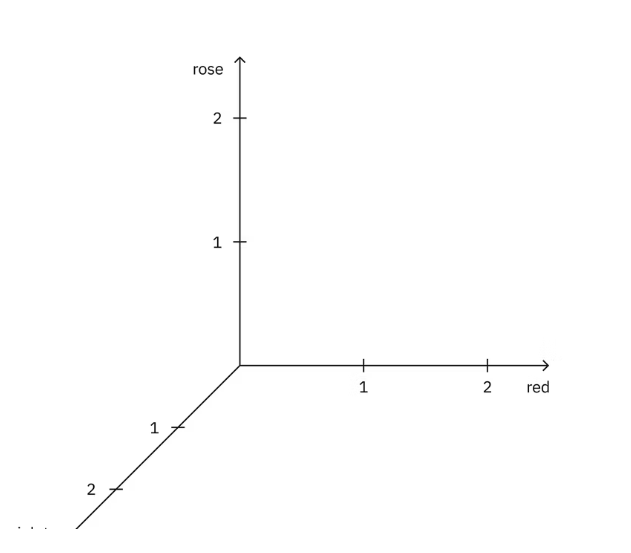
\includegraphics[width=0.4\textwidth]{imagenes/espacioTridimensional} 
    \caption{Representación del espacio tridimensional para el modelo de bolsa de palabras.}
    \label{fig:espacio_3d}
\end{figure}

Dado que rojo, rosa y violeta aparecen una vez en el documento 1, el vector para ese documento será (1,1,1). En el documento 2, rojo aparece dos veces, rosa aparece una vez y violeta no aparece. Por lo tanto, el punto vectorial para el documento 2 es (2,1,0).

\begin{figure}[h]
    \centering
   	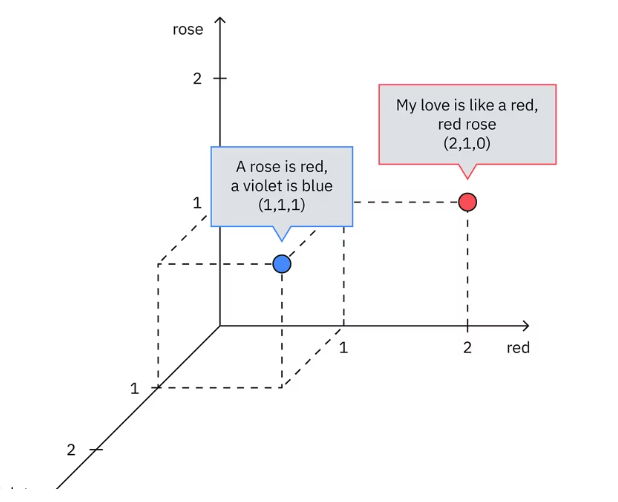
\includegraphics[width=0.4\textwidth]{imagenes/puntosEspacio}
    \caption{Puntos sobre el espacio tridimensional}
    \label{fig:puntos_3d}
\end{figure}

\begin{figure}[h]
    \centering
    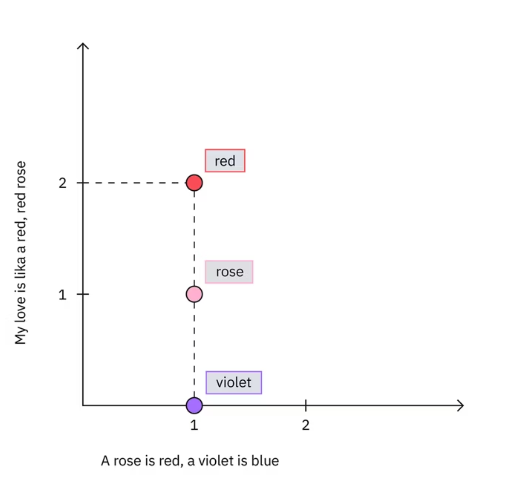
\includegraphics[width=0.4\textwidth]{imagenes/puntosDosDimensiones}
    \caption{Puntos mostrados en un espacio de dos dimensiones}
    \label{fig:puntos_2d}
\end{figure}

Para un modelo de bolsa de palabras, lo único que importa es la cantidad de ocurrencias. Esto nos deja como limitación que todas las palabras tienen la misma importancia.

Trasladando este modelo a la DDP, un documento que contenga los términos 'profesor', 'calificación' y 'extraordinario' se representará como un punto en un espacio donde dichas palabras son dimensiones. Si otra queja presenta una frecuencia similar de estos términos, los puntos resultantes estarán geométricamente cercanos, permitiendo al modelo agruparlas bajo la categoría de competencia académica.

\subsection{TF-IDF (Term Frequency - Inverse Document Frequency)}

Para resolver las limitaciones de BoW, se utilizaría un esquema de pesaje TF-IDF, asignando un valor a cada termino basado no solo en la frecuencia, sino en la relevancia global. Combina dos componentes:

\begin{itemize}
    \item \textbf{Term Frequency (TF):} Mide la frecuencia con la que aparece una palabra en un documento. Una frecuencia más alta sugiere mayor importancia, entonces, si un termino aparece con frecuencia en un documento, es probable que sea relevante para el contenido del documento.
    \begin{equation}
    TF(t,d) = \frac{\text{Número de veces que el término } t \text{ aparece en el documento } d}{\text{Total de términos en el documento } d}
    \end{equation}
    \item \textbf{Inverse Document Frequency (IDF):} Reduce el peso de las palabras comunes en varios documentos y al mismo tiempo aumenta el peso de las palabras raras. Si un termino aparece en menos documentos, es más probables que sea significativo.
    \begin{equation}
    IDF(t, D) = \log\left(\frac{\text{Número total de documentos en el corpus } D}{\text{Número de documentos que contienen el término } t}\right)
    \end{equation}
\end{itemize}
Este equilibrio permite resaltar términos que son frecuentes dentro de un documento especifico, lo que lo convierte en una herramienta útil para tareas de clasificación de texto. 

Esta ponderación es vital para el motor de clasificación, ya que términos genéricos como 'Politécnico' o 'Instituto', que aparecen en casi todas las quejas (IDF bajo), pierden peso frente a términos específicos y raros como 'sindical' o 'laboral' (IDF alto). Esto permite que el sistema ignore el ruido institucional y se centre en las palabras que realmente definen la improcedencia por materia.

\subsection{Modelos de continuidad (Word embeddings)}

En el contexto de la DDP, los word embeddings permiten que el sistema entienda que una queja que menciona 'maltrato docente' es semánticamente similar a una que hable de 'hostigamiento de profesor', aunque no compartan las mismas palabras exactas. Al capturar relaciones complejas, el modelo supera las limitaciones de la coincidencia exacta de términos, reconociendo la intención del quejoso.

Con los Word embeddings asignamos a cada palabra un vector en un espacio de varias dimensiones, con la posición de estos vectores en el espeacio observaríamos la cercanía semántica entre las palabras, por ende, si dos palabras tienen significados similares, sus vectores estarán cercanos.
 
La manera en que se crean los word embeddings consiste en entrenar un modelo en un gran corpus de texto, para así aprender la estructura del lenguaje, esto implica hacer un preprocesamiento en el corpus, en donde tokenizamos las palabras y normalizamos el texto.

Después de haber preprocesado el texto, es necesario hacer uso de una técnica conocida como “ventana de contexto deslizante” para extraer información. Con esto, cada palabra objetivo, se toman en cuenta las palabras que la rodean dentro de un cierto rango, por ende, el modelo será entrenado para aprender a predecir una palabra objetivo usando las palabras de su contexto.
.

\subsubsection{Word2Vec y GloVe (captura de relaciones semánticas mediante contextos locales)}

Son dos modelos que generan representaciones de palabras (word embeddings), utilizan redes neuronales para aprender el contexto de palabras.
Word2Vec es un modelo predictivo que a través de redes neuronales aprende vectores de palabras, se basa en el contexto local de las palabras, ya sea prediciendo palabras de contexto dada una palabra central o viceversa, con este enofque, capturamos relaciones semánticas y sintácticas finas.

GloVe es un modelo basado en conteos, que construye una matriz global de co-ocurrencia que refleja cuantas veces aparecen pares de palabras juntas en todo el corpus. Luego factoriza la matriz para obtener vectores que preservan relaciones estadísticas globales, explícitamente, permite capturar mejor estructuras lineales y relaciones semánticas amplias.

Mientras que TF-IDF solo busca coincidencias exactas de palabras, los embeddings permiten que el sistema entienda que una queja sobre "violencia docente" es semánticamente similar a una de "maltrato de profesor", incluso si no comparten las mismas palabras exactas.


\section{Profundización en el Algoritmo Multinomial Naive Bayes}

Naive Bayes es un modelo bayesiano, es decir, probabilístico. Esto quiere decir que, las predicciones se basan en calcular probabilidades.

Además, tal como su nombre indica, es un modelo Naive, es decir, ingénuo. Esto es porque Naive Bayes asume que el efecto de una variable es independiente al resto de variables. De esta forma, el cálculo de las probabilidades es mucho más sencillo.

En definitiva, si en un mensaje aparece la palabra «buenos» esto será independiente de que aparezce la palabra «días». Como puedes esperar, en la realidad esto no es así. Sin embargo, esta asunción facilita mucho los cálculos, tal como veremos más adelantes.

Y es que, en términos matemáticos, el cálculo matemático de Naive Bayes se traduce en la siguiente fórmula, la cual se conoce como regla de Bayes:

\begin{equation}
P(A|B) = \frac{P(B|A)P(A)}{P(B)}
\end{equation}

Donde: 
\begin{itemize}
\item P(A|B) representa la probabilidad de que ocurra A sabiendo que B ya ha ocurrido.
\item P(B|A) es la probabilidad de que ocurra B sabiendo que se ha dado A.
\item P(A) Probabilidad de que ocurra A.
\item P(B) Probabilidad de que ocurra B.
\end{itemize}



\subsection{Supuesto de independencia condicional (ventajas y desventajas)}

El supuesto central de los clasificadores Naive Bayes es la independencia condicional de las características dada la clase.  Esto significa que, una vez conocida la clase, el valor de una característica no depende del valor de cualquier otra característica. 
Esto significa que:
\begin{equation}
P(x_1, \dots, x_d | y) = \prod_{i=1}^d P(x_i | y)
\end{equation}
Este supuesto simplifica enormemente el cálculo de la probabilidad conjunta, haciendo que el modelo sea computacionalmente eficiente y fácil de entrenar, incluso con grandes cantidades de datos. 

\begin{itemize}
    \item \textbf{Ventajas:} : El modelo es rápido de entrenar e inferir, lo que lo hace ideal para tareas como filtrado de spam o clasificación de texto. 
    \item \textbf{Limitaciones:} En la práctica, las características rara vez son verdaderamente independientes. Por ejemplo, en un correo electrónico, la palabra "oferta" puede estar relacionada con "descuento". A pesar de esto, el clasificador suele funcionar bien en muchos escenarios reales, especialmente con tamaños de muestra pequeños. 
\end{itemize}

En el contexto de la DDP, este supuesto implica que la aparición de la palabra 'sindical' es tratada como independiente de la palabra 'conflicto'. Aunque en la realidad jurídica estas palabras suelen aparecer juntas en casos de improcedencia laboral, Naive Bayes las procesa por separado para simplificar el cálculo probabilístico. A pesar de esta simplificación 'ingenua', el modelo resulta altamente efectivo para identificar patrones léxicos que separan una queja académica de una administrativa.

\subsection{Estimación de máxima verosimilitud}

La Estimación de máxima verosimilitud (MLE) en el clasificador Naive Bayes es un método para estimar los parámetros del modelo, como las probabilidades a priori de las clases y las verosimilitudes de las características dadas una clase, basándose en las frecuencias observadas en el conjunto de entrenamiento. 
\begin{itemize}
    \item \textbf{Prioris de clase:} $P(c) = \frac{\text{número de registros de clase } c}{\text{número total de registros}}$.
    \item \textbf{Verosimilitud:} Para atributos discretos se estima como frecuencia relativa. Para continuos, se asume distribución normal.
\end{itemize}

Este enfoque de MLE es directo y eficiente, pero tiene un problema crítico: si una combinación de clase y característica no aparece en el conjunto de entrenamiento, su probabilidad se estima como cero, lo que puede anular toda la predicción. Para evitar esto, se utilizan técnicas de suavizado (como el suavizado de Laplace), que añaden un valor pequeño (por ejemplo, 1) al numerador y al denominador para evitar ceros. 

\subsection{El problema de la probabilidad cero}


El problema de la probabilidad cero en Naive Bayes surge cuando una característica (por ejemplo, una palabra en texto) no aparece en los datos de entrenamiento para una clase determinada. Esto hace que la probabilidad condicional de esa característica dada la clase sea cero. Como Naive Bayes multiplica todas las probabilidades condicionales para obtener la probabilidad posterior, un valor cero anula completamente el resultado, llevando a predicciones incorrectas o imposibles, incluso si otras características indican claramente la clase correcta.

Para la Defensoría, este problema es crítico. Si una queja nueva contiene una palabra jurídica poco común o un término técnico específico que no figuraba en el histórico de entrenamiento, el modelo podría asignar una probabilidad de cero a la clase 'Competente', rechazando la queja automáticamente de forma errónea. La implementación del suavizado de Laplace es, por tanto, una salvaguarda procedimental que garantiza que ningún término nuevo anule la posibilidad de que un ciudadano sea atendido.

La técnica más utilizada para resolver este problema es el suavizado de Laplace (también llamado suavizado aditivo).  Consiste en sumar un valor pequeño (generalmente 1) al recuento de cada combinación de clase y característica, asegurando que ninguna probabilidad sea cero. Esto permite que el modelo haga predicciones incluso para características nuevas o raras.

La fórmula ajustada para el suavizado de Laplace se expresa de la siguiente manera:
\begin{equation}
\hat{P}(x_i | c) = \frac{N_{x_i,c} + \alpha}{N_c + \alpha d}
\end{equation}

Donde:
\begin{itemize}
    \item $N_{x_i,c}$ es el recuento de la característica $x_i$ en la clase $c$.
    \item $N_c$ es el total de características en la clase $c$.
    \item $d$ es el número de características posibles (tamaño del vocabulario).
    \item $\alpha$ es el parámetro de suavizado (comúnmente se utiliza $\alpha = 1$).
\end{itemize}

Este ajuste mejora la generalización del modelo y evita que el clasificador se rompa ante datos no vistos en el entrenamiento.

Mientras que Naive Bayes ofrece una solución basada en la frecuencia de términos y la actualización de creencias probabilísticas, presenta limitaciones cuando las palabras clave de ambas clases (competente e improcedente) se traslapan significativamente. Para abordar estas fronteras de decisión más complejas, se introduce a continuación el modelo de Máquinas de Soporte Vectorial (SVM).

\section{Support Vector Machines}


Una Support Vector Machine es un algoritmo de Machine Learning supervisado que se suele utilizar para problemas de clasificación y regresión en aplicaciones de procesamiento de señales, procesamiento del lenguaje natural (PLN), y reconocimiento del habla e imágenes. El objetivo del algoritmo de SVM es encontrar un hiperplano que, en la mejor medida posible, separe los puntos de datos de una clase de los de otra clase. Este hiperplano puede ser una línea para espacio en 2D o un plano para un espacio con n dimensiones, donde n es el número de características de cada observación del conjunto de datos. Pueden existir múltiples hiperplanos que separen las clases de los datos. El hiperplano óptimo, derivado por el algoritmo de SVM, es el que aumenta el margen entre las dos clases.

El margen es la anchura máxima de la franja paralela al hiperplano que no contiene puntos de datos en su interior. Los puntos de datos que marcan el límite de esta franja paralela y están más cerca del hiperplano separador son los vectores de soporte. Los vectores de soporte hacen referencia a un subconjunto de las observaciones de entrenamiento que determinan la ubicación del hiperplano separador.

El hiperplano óptimo representa la frontera de decisión legal. Los vectores de soporte serían aquellas quejas cuyas narrativas son más ambiguas o se encuentran en el límite de la competencia (por ejemplo, casos que rozan lo laboral pero mantienen un componente de derechos politécnicos). Maximizar el margen asegura que el sistema sea robusto y no clasifique erróneamente una queja debido a pequeñas variaciones en el vocabulario del quejoso."

\subsection{Optimización de hiperplano de separación (margen máximo)}

La Máquina de Vectores de Soporte (SVM) busca encontrar el hiperplano de separación óptimo que maximice el margen entre las clases; es decir, la distancia entre el hiperplano y los puntos de datos más cercanos de cada clase, conocidos como \textbf{vectores de soporte}.

El objetivo del problema de optimización en SVM se formula como:

\begin{itemize}
    \item \textbf{Maximizar el margen:} Equivalente a minimizar $\|w\|$, donde $w$ es el vector normal al hiperplano.
    \item \textbf{Sujeto a las restricciones:} Para cada dato $(x_i, y_i)$, se debe cumplir que $y_i(\langle w, x_i \rangle + b) \geq 1$, donde $y_i \in \{-1, +1\}$ es la etiqueta de clase.
\end{itemize}

Este problema se resuelve mediante optimización dual usando multiplicadores de Lagrange, lo que permite obtener la solución mediante el lagrangiano dual, donde solo los vectores de soporte (aquellos con $\alpha_i > 0$) influyen en el hiperplano final. Para datos no linealmente separables, se introduce una variable de holgura $\xi_i$ y un parámetro de regularización $C$, que controla el \textit{trade-off} entre:

\begin{itemize}
    \item \textbf{Máximo margen:} Menor complejidad y mayor capacidad de generalización.
    \item \textbf{Menos errores de clasificación:} Mayor ajuste al conjunto de entrenamiento.
\end{itemize}

El hiperplano final de decisión se define mediante la siguiente función:

\begin{equation}
f(x) = \text{sign} \left( \sum_{i=1}^{n} \alpha_i y_i K(x_i, x) + b \right)
\end{equation}

\noindent donde los coeficientes $\alpha_i$ se obtienen de la formulación dual. En la biblioteca \textit{scikit-learn}, la clase \texttt{SVC} implementa esta optimización con parámetros clave:

\begin{itemize}
    \item \textbf{$C$:} Controla el balance entre la amplitud del margen y los errores permitidos.
    \item \textbf{\textit{Kernel}:} Define el tipo de transformación (lineal, polinomial o RBF).
    \item \textbf{\textit{Gamma}:} Para \textit{kernels} como RBF, afecta la flexibilidad del modelo y el alcance de influencia de un solo ejemplo de entrenamiento.
\end{itemize}

\subsection{Flexibilidad mediante variables de holgura}

Las variables de holgura juegan un papel importante en las máquinas de vectores de soporte de margen suave (\textit{Soft Margin} SVM). Para comprender su importancia, es necesario considerar primero el concepto de margen suave.

En escenarios del mundo real, a menudo no es posible encontrar un hiperplano que separe perfectamente los datos. Aquí es donde entra en juego la SVM de margen suave, la cual permite cierta clasificación errónea de puntos de datos mediante la introducción de un término de penalización controlado por un hiperparámetro denominado parámetro de regularización ($C$). Un valor mayor de $C$ indica una sanción mayor por clasificación errónea, lo que da como resultado un margen más estrecho; por el contrario, un valor más pequeño de $C$ permite una mayor tolerancia al error, lo que conduce a un margen más amplio.



El papel de las variables de holgura ($\xi_i$) es manejar puntos de datos mal clasificados o que se encuentran dentro del margen. Estas variables representan la distancia de un punto que viola el margen desde su límite de clase correcto. En consecuencia, el problema de optimización se formula con restricciones de la siguiente forma:

\begin{equation}
\min \quad \frac{1}{2} \|w\|^2 + C \sum_{i=1}^{n} \xi_i
\end{equation}

\noindent sujeto a las restricciones:

\begin{itemize}
    \item $y_i(w^T x_i + b) \geq 1 - \xi_i$ para todo $i$.
    \item $\xi_i \geq 0$ para todo $i$.
\end{itemize}

En esta formulación, $w$ representa el vector de peso, $b$ es el término de sesgo, $x_i$ es el vector de entrada, $y_i$ es la etiqueta de clase correspondiente y $\xi_i$ es la variable de holgura asociada con el $i$-ésimo ejemplo de entrenamiento. 

El término $\frac{1}{2} \|w\|^2$ representa el margen y el término $C \sum \xi_i$ representa la penalización por clasificación incorrecta. Las restricciones aseguran que los puntos de datos se clasifiquen correctamente, con un margen de al menos $1 - \xi_i$. De esta manera, las variables de holgura permiten cierta flexibilidad, logrando un equilibrio entre maximizar el margen y minimizar el error. 

Considerando un ejemplo donde las clases no son linealmente separables, una SVM de margen blando con la elección adecuada de estas variables puede encontrar un hiperplano funcional para la DDP con cierta tolerancia a la clasificación errónea, ayudando a cuantificar el alcance de las infracciones y ajustando el margen en consecuencia.

\subsection{El truco kernel}

El truco del kernel es un concepto fundamental en los algoritmos de la máquina de vectores de soporte (SVM) que permite el manejo de datos complejos transformándolos en un espacio de características de mayor dimensión. Esta técnica es particularmente útil cuando se trata de datos separables de forma no lineal, ya que permite que las SVM clasifiquen dichos datos de manera efectiva asignándolos implícitamente a un espacio de mayor dimensión.
Para comprender el truco del kernel, primero revisemos la idea básica detrás de las SVM. Las SVM son modelos de aprendizaje supervisado que tienen como objetivo encontrar un hiperplano óptimo que separe los puntos de datos que pertenecen a diferentes clases. En el caso de datos linealmente separables, un hiperplano lineal puede separar perfectamente las clases. Sin embargo, cuando los datos no son linealmente separables, las SVM emplean una función kernel para mapear los datos en un espacio de mayor dimensión donde la separación lineal es posible.
Una función central es una función matemática que toma dos vectores de entrada y calcula su similitud o producto interno en el espacio de características de dimensiones superiores. Permite que las SVM operen en el espacio de entrada original sin calcular explícitamente la transformación al espacio de dimensiones superiores. Esto es importante porque el cálculo explícito de la transformación podría resultar costoso o incluso imposible para ciertos tipos de transformaciones.
Al usar el truco del kernel, las SVM pueden calcular de manera eficiente el límite de decisión en el espacio de características de mayor dimensión sin transformar explícitamente los datos. Esto se logra definiendo la función kernel para calcular implícitamente el producto interno entre los vectores de características transformados. El algoritmo SVM solo necesita calcular la función kernel para pares de vectores de entrada, en lugar de calcular la transformación para todos los puntos de datos individuales.
Hay varios tipos de funciones de kernel que se usan comúnmente en las SVM, incluidas las funciones lineales, polinómicas, de base radial gaussiana (RBF) y kernels sigmoides. Cada función del núcleo tiene sus propias características y la elección del núcleo depende del problema específico y la naturaleza de los datos.
Por ejemplo, el kernel lineal simplemente calcula el producto interno entre los vectores de entrada, realizando efectivamente una clasificación lineal en el espacio de entrada original. El núcleo polinomial eleva el producto interno a una cierta potencia, lo que permite límites de decisión no lineales. El kernel RBF mide la similitud entre dos vectores en función de su distancia euclidiana, lo que permite que las SVM capturen patrones complejos en los datos. El kernel sigmoide calcula la tangente hiperbólica del producto interno, lo que puede ser útil en ciertos escenarios.
Debido a que el lenguaje humano es inherentemente no lineal —donde la combinación de palabras cambia el sentido de forma compleja—, el uso de un Kernel RBF o Polinomial permite que el motor de la DDP proyecte las quejas en un espacio de dimensiones superiores. Esto facilita encontrar separaciones que en el espacio original de palabras (BoW) serían imposibles de trazar.

\subsection{Enfoque matemático}

Para comenzar, el \textit{kernel} es un modelo para abordar la no linealidad siendo este un algoritmo discriminativo. Pero, ¿cómo funciona? Partimos de una configuración de regresión simple:

\begin{figure}[h]
    \centering
   	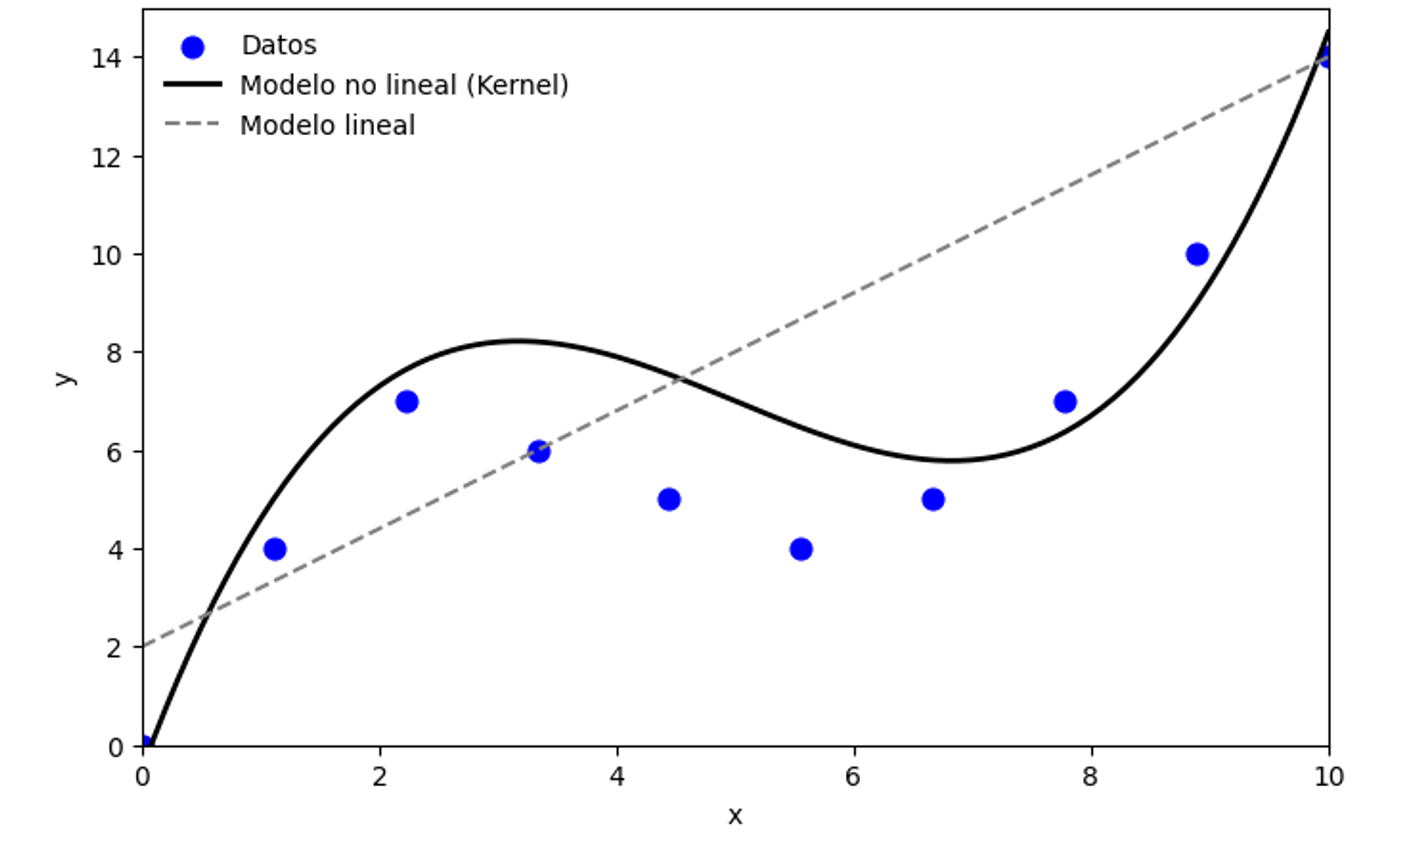
\includegraphics[width=0.4\textwidth]{imagenes/metodoKernel}
    \label{fig:metodo_kernel}
    \caption{Gráfica que representa datos no lineales}
\end{figure}

Si observamos los datos como un modelo lineal, estaríamos cometiendo un error; podemos interpretar los datos mediante una función polinomial cúbica con el fin de ajustarlos. Sea $h(x)$ mi modelo, siendo $x \in \mathbb{R}$ por simplicidad:

\[ h(x) = \theta_0 + \theta_1 x + \theta_2 x^2 + \theta_3 x^3 \]

Teniendo así un modelo no lineal en $x$, pero sí lineal en $\theta$. Esto es fundamental, ya que la linealidad en los parámetros es suficiente para aplicar técnicas conocidas. Podemos convertir esto a una Regresión Lineal estándar definiendo el vector de características:

\[ \phi(x) = \begin{bmatrix} 1 \\ x \\ x^2 \\ x^3 \end{bmatrix} \]

Reescribiendo así el modelo no lineal a uno lineal:

\[ h(x) = \theta^T \phi(x) \]

Con esto, el modelo es lineal en $\theta$ y lineal en las coordenadas $\phi(x)$. Antes la entrada era unidimensional, pero con $\phi(x)$ tenemos un vector de $p=4$ dimensiones. Si nuestro dataset original era $\{x_1, x_2, \dots, x_n\}$, el nuevo dataset estará compuesto por $\{\phi(x_1), \phi(x_2), \dots, \phi(x_n)\}$.

Al aplicar el \textbf{descenso del gradiente} para minimizar la función de pérdida:

\[ J(\theta) = \frac{1}{2} \sum_{i=1}^{n} (h(x_i) - y_i)^2 \]

En el caso estándar, el algoritmo de actualización es:

\[ \theta_{t+1} = \theta_t - \alpha \nabla J(\theta_t) \]
\[ \theta_{t+1} = \theta_t - \alpha \sum_{i=1}^n (\theta_t^T \phi(x_i) - y_i) \phi(x_i) \]

¿Cuál es la dimensión de $\theta$? Es la misma que la de $\phi(x)$, es decir, $p$. Si $p$ es muy alto (por ejemplo, con monomios de alto grado), el costo de operación $O(p)$ por cada actualización vuelve al algoritmo ineficiente. 

Para acelerar esto, aplicamos el \textbf{truco del kernel}. Observamos que $\theta$ puede representarse como una combinación lineal de las características de entrenamiento:

\[ \theta = \sum_{i=1}^n \beta_i \phi(x_i) \]

Donde $\beta$ es un vector de $n$ dimensiones (el número de datos). Si inicialmente $\theta_0 = 0$, en cada iteración $t$:

\[ \theta_{t+1} = \sum_{i=1}^n \beta_i^{(t+1)} \phi(x_i) \]

Sustituyendo esto en la regla de actualización, podemos encontrar cómo evoluciona $\beta$ sin necesidad de calcular $\theta$ explícitamente:

\[ \beta_j^{(t+1)} = \beta_j^{(t)} - \alpha \left( \sum_{i=1}^n \beta_i^{(t)} \phi(x_i)^T \phi(x_j) - y_j \right) \]

Para que esto sea eficiente, introducimos la función Kernel $K(x, z) = \phi(x)^T \phi(z)$. Por ejemplo, si:
\[ \phi(x) = \begin{bmatrix} x_1^3 \\ x_1^2 x_2 \\ \vdots \end{bmatrix} \]

El producto interno en un espacio de alta dimensión $p$ es costoso, pero si existe una función $K(x, z)$ tal que:
\[ K(x, z) = (x^T z + c)^d \]
Entonces calcular el producto interno toma tiempo $O(d)$ (dimensión original) en lugar de $O(p)$.

\textbf{Método de kernel para regresión:}

1. Precalcular la matriz de Kernel $K_{ij} = K(x_i, x_j)$ para todo $i, j = 1, \dots, n$. Esto toma $O(n^2 d)$.
2. Inicializar $\beta^{(0)} = 0$.
3. Bucle de actualización:
\[ \beta_j^{(t+1)} = \beta_j^{(t)} - \alpha \left( \sum_{i=1}^n \beta_i^{(t)} K_{ij} - y_j \right) \]

Este algoritmo tiene una complejidad por iteración de $O(n^2)$, lo cual es mucho mejor que $O(np)$ siempre que $n < p$.


\section{Estrategias de entrenamiento y validación}

\subsection{Manejo de clases desbalanceadas}
El desbalance de clases ocurre cuando la distribución de las etiquetas de salida es significativamente asimétrica. Un modelo entrenado bajo estas condiciones tenderá a maximizar la exactitud global simplemente prediciendo la clase mayoritaria, ignorando los casos minoritarios (que suelen ser los de mayor interés, como el fraude o enfermedades raras).

\begin{itemize}
\item \textbf{Random Undersampling:} Consiste en eliminar aleatoriamente ejemplos de la clase mayoritaria para igualar la proporción de la minoritaria. Aunque reduce el tiempo de cómputo, existe el riesgo de descartar información valiosa que define los límites de decisión de la clase dominante.
\item \textbf{SMOTE (Synthetic Minority Over-sampling Technique):} En lugar de duplicar registros existentes, SMOTE genera nuevas instancias sintéticas. El algoritmo selecciona un punto de la clase minoritaria, identifica sus $k$ vecinos más cercanos y traza segmentos de línea entre ellos, creando nuevos puntos sobre dichos segmentos. Esto expande la región de decisión de la clase minoritaria de forma coherente.

\end{itemize}

\subsection{Optimización de hiperparámetros}

A diferencia de los parámetros (como los pesos $\theta$ que el modelo aprende por sí mismo), los hiperparámetros son configuraciones externas que definen el comportamiento del algoritmo de aprendizaje.

\begin{itemize}
\item \textbf{SVM y el parámetro $C$:} Regula el \textit{trade-off} entre el margen de decisión y el error de clasificación. Un $C$ pequeño permite un margen más amplio aceptando algunos errores (sesgo alto, varianza baja), mientras que un $C$ grande intenta clasificar todos los puntos correctamente, arriesgando el sobreajuste (\textit{overfitting}).

\item \textbf{Naive Bayes y el suavizado de Laplace ($\alpha$):} Evita el problema de la "probabilidad cero". Si una palabra no aparece en el entrenamiento para una clase específica, la probabilidad sería $0$, anulando todo el producto. $\alpha$ añade un conteo pequeño a todas las frecuencias para garantizar estabilidad numérica.

\item \textbf{Grid Search vs. Random Search:} Mientras que Grid Search evalúa todas las combinaciones posibles en un rango definido (exhaustivo pero lento), Random Search selecciona combinaciones al azar, lo que suele ser más eficiente para encontrar zonas de optimización en espacios de alta dimensión.
\end{itemize}

\subsection{Validación cruzada (K-Fold Cross-Validation)}
Para obtener una estimación robusta del rendimiento y evitar que la métrica dependa de una partición de datos "afortunada", se utiliza K-Fold. El dataset se divide en $K$ subconjuntos iguales (folds). 
El proceso se repite $K$ veces:\begin{enumerate}
\item Se reserva el fold $k$ para validación.
\item Se entrena el modelo con los $K-1$ restantes.
\item Se calcula la métrica en el fold de validación.
\end{enumerate}
Al final, el rendimiento reportado es el promedio de las $K$ iteraciones:$$E_{total} = \frac{1}{K} \sum_{i=1}^{K} E_i$$


\section{Evaluación de la inteligencia del sistema}
Para medir la eficacia real, especialmente en sistemas no balanceados, no basta con la exactitud. Debemos recurrir a la \textbf{Matriz de Confusión}, que clasifica los resultados en Verdaderos Positivos (VP), Falsos Positivos (FP), Verdaderos Negativos (VN) y Falsos Negativos (FN).
\begin{itemize}
\item \textbf{Accuracy (Exactitud):} Representa la fracción total de predicciones correctas. Es engañosa si las clases están desbalanceadas.
$$\text{Accuracy} = \frac{VP + VN}{VP + VN + FP + FN}$$
\item \textbf{Precisión (Valor Predictivo Positivo):} Responde a: "¿De todas las veces que el sistema predijo 'Queja', cuántas realmente lo eran?". Es crítica cuando el costo de un Falso Positivo es alto.
$$\text{Precisión} = \frac{VP}{VP + FP}$$
\item \textbf{Recall (Sensibilidad):} Responde a: "¿De todas las quejas reales que existían, cuántas logró detectar el sistema?". Es vital cuando no podemos permitirnos omitir casos (Falsos Negativos).
$$\text{Recall} = \frac{VP}{VP + FN}$$
\item \textbf{F1-Score:} Es la media armónica de la precisión y el recall. Penaliza valores extremos, siendo una métrica excelente para encontrar un equilibrio entre ambas.
$$F1 = 2 \cdot \frac{\text{Precisión} \cdot \text{Recall}}{\text{Precisión} + \text{Recall}}$$
\item \textbf{Curvas ROC y AUC:} La curva ROC (\textit{Receiver Operating Characteristic}) grafica la Tasa de Verdaderos Positivos frente a la Tasa de Falsos Positivos al variar el umbral de clasificación. El área bajo la curva (AUC) mide la capacidad del modelo para distinguir entre clases; un AUC de 1.0 es perfecto, mientras que 0.5 equivale a una clasificación aleatoria.
\end{itemize}


\section{Selección de Tecnologías}


\subsection{Definición de arquitectura de software}
La arquitectura de software se entiende como el conjunto de patrones y abstracciones que proporcionan el marco de referencia necesario para llevar a cabo la construcción de un sistema. Funciona como el esqueleto del software...

\subsection{Arquitectura del Sistema}

\begin{flushleft}
\section{Definición de arquitectura de software}
\end{flushleft}
\justifying
La arquitectura de software se entiende como el conjunto de patrones y abstracciones que proporcionan el marco de referencia necesario para llevar a cabo la construcción de un sistema. Funciona como el esqueleto del software, ya que en este se define cómo se organizan los componentes, cómo interactúan entre sí y bajo qué principios se rigen para cumplir con los objetivos del negocio [13]. 
\subsection{Importancia en el desarrollo de sistemas}

La importancia de la arquitectura de software radica en que permite a los equipos de desarrollo tener una visión clara y compartida de la solución, facilitando la toma de decisiones críticas antes de iniciar la etapa de codificación detallada. Sin embargo, su relevancia se extiende a múltiples dimensiones estratégicas del ciclo de vida del software:

\begin{itemize}
    \item \textbf{Gestión de la Complejidad:} En sistemas modernos, la arquitectura actúa como un mapa conceptual que divide el sistema en componentes manejables. Esto permite a los desarrolladores centrarse en módulos específicos sin perder de vista la interacción global, reduciendo la carga cognitiva y el riesgo de errores por efectos secundarios.
    
    \item \textbf{Mitigación de Riesgos Tempranos:} Permite identificar cuellos de botella potenciales, fallos de seguridad o limitaciones de rendimiento en las fases de diseño. Es significativamente más económico corregir un error estructural en un diagrama arquitectónico que refactorizar miles de líneas de código una vez que el sistema está en producción.
    
    \item \textbf{Base para la Escalabilidad y Mantenibilidad:} Una arquitectura bien definida prevé el crecimiento futuro del sistema. Establece las reglas para añadir nuevas funcionalidades o integrar servicios de terceros sin degradar la integridad de la solución original, garantizando que el software pueda evolucionar de forma sostenible.
    
    \item \textbf{Facilitación del Consenso entre Interesados:} Sirve como un lenguaje común entre perfiles técnicos (desarrolladores, DevOps) y no técnicos (clientes, gerentes de producto). Al visualizar la estructura, todos los \textit{stakeholders} pueden validar si los requisitos de negocio se están traduciendo correctamente en soluciones técnicas.
    
    \item \textbf{Guía para la Toma de Decisiones:} Proporciona el marco de referencia necesario para elegir el \textit{stack} tecnológico adecuado (bases de datos, lenguajes, frameworks) y para gestionar los \textit{trade-offs} o compromisos técnicos, como decidir entre priorizar la latencia mínima o la consistencia absoluta de los datos.
\end{itemize}

En definitiva, la arquitectura no es solo un artefacto técnico, sino el cimiento que asegura que el equipo no solo construya el sistema correctamente, sino que construya el sistema \textit{adecuado} para las necesidades del negocio.


\subsection{Factores de calidad}

Para asegurar que la estructura seleccionada sea la adecuada, esta debe ser evaluada bajo atributos de calidad que garanticen su viabilidad a largo plazo. De acuerdo con los modelos de calidad internacionales como el ISO/IEC 9126 (y su evolución en la norma ISO/IEC 25010), estos atributos permiten medir la capacidad del software para satisfacer necesidades explícitas e implícitas bajo condiciones determinadas [14]. En el contexto de un sistema de gestión institucional de denuncias, destacan los siguientes pilares:

\begin{itemize}
    \item \textbf{Rendimiento y Eficiencia:} Evalúa el comportamiento temporal del sistema y la utilización óptima de recursos al procesar transacciones. En una arquitectura de microservicios, esto implica garantizar latencias mínimas en la comunicación entre servicios (vía API REST) para que la experiencia del usuario sea fluida, incluso durante procesos complejos de carga de evidencias o archivos adjuntos [14].
    
    \item \textbf{Mantenibilidad:} Representa la facilidad con la que el software puede ser modificado para corregir defectos, mejorar el desempeño o adaptarse a cambios normativos en el IPN. Gracias al uso de \textit{Docker} y una estructura de tres capas, el sistema permite que cada microservicio sea actualizado de forma independiente, reduciendo el riesgo de introducir errores en módulos no relacionados y garantizando la estabilidad operativa [14].

    \item \textbf{Escalabilidad (Horizontal y Vertical):} Es la capacidad del sistema para ajustarse a variaciones en la demanda de procesamiento. Para la Defensoría, esto es vital en periodos de alta afluencia de usuarios; la arquitectura permite realizar un escalado horizontal (añadir más instancias de un microservicio crítico como el de denuncias) sin necesidad de replicar toda la aplicación, optimizando el uso de la infraestructura institucional [15].

    \item \textbf{Seguridad y Confidencialidad:} Dado el carácter sensible de las quejas procesadas, este atributo asegura que la información solo sea accesible por personal autorizado mediante esquemas de RBAC (Control de Acceso Basado en Roles). La arquitectura debe garantizar el cifrado de datos en reposo y en tránsito, protegiendo la identidad del denunciante y la integridad del expediente digital.

    \item \textbf{Disponibilidad y Tolerancia a Fallos:} Asegura que el servicio permanezca operativo la mayor parte del tiempo posible. El enfoque de microservicios previene que la caída del clasificador de texto (Python) afecte el funcionamiento del módulo de gestión de usuarios (Java), permitiendo que el sistema degrade sus funciones de manera elegante en lugar de sufrir un colapso total.
\end{itemize}

La evaluación constante de estos factores permite que la plataforma no solo cumpla con sus requerimientos funcionales, sino que se consolide como una herramienta robusta, confiable y con una vida útil prolongada dentro del ecosistema digital del Instituto.

\subsection{Clasificación de arquitecturas}

Históricamente, las arquitecturas se han clasificado según la forma en que distribuyen sus responsabilidades y cómo gestionan el flujo de datos. De acuerdo con la literatura clásica y los referentes actuales de la industria, destacan las siguientes categorías fundamentales:

\begin{itemize}
    \item \textbf{Arquitecturas Monolíticas:} Representan el modelo tradicional de diseño donde todos los componentes funcionales (interfaz, lógica y datos) se integran en una unidad lógica única con una base de código compartida. Este enfoque facilita el despliegue inicial, pero presenta desafíos críticos de escalabilidad: si un servicio popular requiere más recursos, se debe escalar toda la aplicación innecesariamente, consumiendo recursos de servidor de forma ineficiente. Además, constituye un punto único de fallo, donde un error en cualquier módulo puede provocar la caída total del sistema.

    \item \textbf{Arquitecturas Distribuidas:} Son colecciones de computadores independientes que aparecen ante el usuario como un único sistema coherente. En este modelo, los componentes de hardware y software se comunican y coordinan exclusivamente mediante el paso de mensajes. Su objetivo primordial es compartir recursos e información, logrando una mayor tolerancia a fallos y permitiendo el uso de procesadores poderosos a un menor costo comparativo.

    \item \textbf{Arquitecturas de Microservicios:} Evolución que descompone una aplicación en servicios pequeños, autónomos y altamente cohesivos que pueden ser desarrollados, probados y escalados de forma independiente. Este patrón permite reducir la complejidad operativa y ganar agilidad en la innovación al permitir que diferentes equipos utilicen diversos \textit{stacks} tecnológicos (como Java y Python) de manera simultánea. Se comunican mediante protocolos ligeros, facilitando el despliegue continuo sin interrumpir el funcionamiento global de la plataforma.

    \item \textbf{Arquitecturas por Capas (N-Layer):} Este estilo organiza el software en una distribución jerárquica de roles para proporcionar una división efectiva de problemas. Se basa en el principio de que las capas inferiores no dependen de las superiores, comunicándose mediante interfaces bien definidas para lograr un bajo acoplamiento. Facilita el aislamiento de cambios, permitiendo realizar actualizaciones internas en una capa (como la de persistencia de datos) sin afectar al resto del sistema.

    \item \textbf{Arquitectura Orientada a Eventos (EDA):} Modelo centrado en la producción y consumo de eventos para articular reglas de negocio. En este esquema, el flujo de trabajo es activado por cambios significativos de estado, lo que permite una alta capacidad de respuesta y trazabilidad de las acciones del usuario. Es fundamental en sistemas que requieren una gestión dinámica de elementos basándose en sucesos producidos durante la ejecución.
\end{itemize}


\section{Arquitectura del Sistema}

Para el desarrollo de la "Plataforma Web para la Denuncia Segura y Prevención de Riesgos Digitales", se ha seleccionado una arquitectura de microservicios, la cual se complementa internamente con un patrón de tres capas para la organización de cada servicio. Esta decisión técnica no es arbitraria; se fundamenta en la necesidad de superar las limitaciones de las arquitecturas monolíticas tradicionales, donde el alto acoplamiento entre componentes suele derivar en dificultades para el mantenimiento y la escalabilidad ante una demanda creciente [1].

Al adoptar un enfoque de microservicios, el sistema se descompone en unidades funcionales autónomas que se comunican a través de protocolos ligeros. Según Villamizar et al., esta estructura permite que cada componente evolucione de manera independiente, facilitando la innovación tecnológica y permitiendo que fallos en un servicio específico (como el procesador de lenguaje natural en Python) no comprometan la disponibilidad global de la plataforma administrativa en Java [1].

La organización interna de estos servicios sigue el patrón de tres capas, el cual establece una división clara de responsabilidades:
\begin{itemize}
    \item \textbf{Capa de Presentación:} Gestiona la interacción con el usuario (Angular).
    \item \textbf{Capa de Negocio (Dominio):} Implementa las reglas institucionales de la Defensoría, aislando la lógica de cualquier dependencia externa [3][5].
    \item \textbf{Capa de Acceso a Datos (Infraestructura):} Encargada de la persistencia en PostgreSQL de forma transparente para el resto del sistema [3].
\end{itemize}

Esta arquitectura híbrida garantiza los siguientes pilares fundamentales para el Instituto Politécnico Nacional:
\begin{itemize}
    \item \textbf{Escalabilidad Eficiente:} Siguiendo los principios de sistemas distribuidos, es posible asignar recursos de servidor de manera granular únicamente a los microservicios que presenten mayor carga de trabajo [2].
    \item \textbf{Mantenibilidad y Desacoplamiento:} El uso de capas asegura que cambios en la lógica de negocio o en el motor de base de datos se realicen con un impacto mínimo en el código fuente, reduciendo la deuda técnica a largo plazo [3].
    \item \textbf{Alto Rendimiento:} La distribución de tareas entre nodos independientes y el uso de un proxy inverso optimizan los tiempos de respuesta ante múltiples peticiones concurrentes [2][4].
\end{itemize}


\subsection{Arquitectura de Microservicios}

La arquitectura de microservicios se define como un enfoque de desarrollo de software donde una aplicación se descompone en un conjunto de servicios pequeños, autónomos y altamente cohesivos. Cada uno de estos componentes se ejecuta como un proceso independiente y se comunica con los demás a través de mecanismos ligeros, generalmente interfaces de programación de aplicaciones (APIs) basadas en el protocolo HTTP. A diferencia de las arquitecturas monolíticas, donde una falla en un módulo puede comprometer la totalidad del sistema, los microservicios permiten que cada unidad funcional se enfoque en una capacidad específica del negocio, facilitando su desarrollo, despliegue y escalado de forma totalmente autónoma [1][18].



\textbf{Ventajas de su Uso:}
\begin{itemize}
    \item \textbf{Aislamiento y Resiliencia ante Fallos:} Dado que cada servicio opera en un entorno de ejecución separado, un error crítico o una excepción no controlada en un módulo específico no provoca un efecto dominó sobre el resto de la plataforma. Esta característica es vital para mantener la alta disponibilidad requerida en entornos institucionales [1][18].
    
    \item \textbf{Escalabilidad Granular y Eficiente:} Permite realizar un escalado horizontal selectivo. En lugar de replicar la aplicación completa, es posible asignar recursos de infraestructura adicionales únicamente a aquellos servicios que experimentan una alta demanda de procesamiento, optimizando significativamente el uso del hardware y los costos operativos [1][2].
    
    \item \textbf{Heterogeneidad Tecnológica:} Facilita el uso de diferentes lenguajes de programación y bases de datos según las necesidades específicas de cada módulo. En este proyecto, dicha flexibilidad permite la coexistencia de servicios robustos en Java con módulos especializados en análisis de datos desarrollados en Python [1].
    
    \item \textbf{Agilidad en el Despliegue Continuo:} Al reducir el acoplamiento entre funciones, se acortan los ciclos de desarrollo y se permite la actualización constante de módulos individuales sin necesidad de reiniciar o interrumpir la operación global del sistema [1].
\end{itemize}

\textbf{Justificación para la Defensoría de los Derechos Politécnicos:}
La elección de este enfoque para la plataforma de denuncia segura responde a la complejidad intrínseca de los procesos administrativos y legales del Instituto. El sistema requiere gestionar múltiples roles y flujos de trabajo (denunciantes, abogados, administradores) que poseen demandas computacionales distintas. Se adoptó esta arquitectura para asegurar la continuidad operativa: si el microservicio encargado del procesamiento de lenguaje natural llegara a saturarse, los módulos de registro de quejas y gestión de expedientes continuarían funcionando de forma ininterrumpida. Esta independencia garantiza que la atención a la comunidad politécnica no se vea comprometida por incidentes técnicos aislados en subcomponentes del sistema.


\subsection{Arquitectura Interna de los Servicios: Patrón de 3 Capas}

La arquitectura de tres niveles (o capas) es un modelo de diseño de software cuya finalidad primordial es la separación de las responsabilidades y el desacoplamiento de las etapas de procesamiento de una aplicación. Esta estructura organiza el software en tres niveles lógicos y físicos claramente diferenciados: el nivel de presentación, el nivel de aplicación (o lógica de negocio) y el nivel de datos [3][19]. En este proyecto, dicha estructura conforma de manera exacta el diseño interno de cada microservicio, garantizando que la lógica institucional esté aislada de las interfaces de usuario y de los motores de persistencia.



\begin{itemize}
    \item \textbf{Nivel de Presentación (Interfaz de Usuario):} Es la capa más externa del servicio, encargada de la interacción directa con el usuario o con otros servicios externos. Su función principal es presentar la información y recolectar datos de entrada para enviarlos a la capa de aplicación. Al estar desacoplada, permite realizar cambios estéticos o funcionales en la interfaz (Angular) sin alterar las reglas de negocio subyacentes [3][19].
    
    \item \textbf{Nivel de Aplicación (Lógica de Negocio):} Considerado el núcleo del servicio, es donde se modelan las reglas del negocio y se toman las decisiones lógicas. Según Coti Colop, la ubicación de las reglas en esta capa central es crítica para asegurar la funcionalidad y la integridad del sistema, ya que actúa como un puente que coordina las peticiones de la interfaz y la gestión de los datos, protegiendo la coherencia de los procesos legales y administrativos de la Defensoría [5].
    
    \item \textbf{Nivel de Datos (Persistencia):} Es la capa responsable del almacenamiento y la recuperación de la información. Gestiona la comunicación con el Sistema de Gestión de Bases de Datos (PostgreSQL), permitiendo que la persistencia sea transparente para las capas superiores. Esto significa que el motor de base de datos podría ser optimizado o sustituido con un impacto mínimo en la lógica de negocio [19].
\end{itemize}

\textbf{Ventajas de su Uso:}
\begin{itemize}
    \item \textbf{Independencia y Escalabilidad:} Cada nivel puede ser escalado de forma independiente según la demanda específica. Por ejemplo, si el procesamiento de datos aumenta, se puede fortalecer la capa de aplicación sin necesidad de modificar la interfaz de usuario [3][19].
    \item \textbf{Mantenibilidad y Flexibilidad:} Facilita el mantenimiento a largo plazo al permitir que cada capa sea desarrollada, probada y actualizada simultáneamente por distintos integrantes del equipo, lo que reduce significativamente el tiempo total de desarrollo y el riesgo de introducir errores colaterales [19].
    \item \textbf{Confiabilidad Operativa:} Al operar de manera aislada, una interrupción o fallo en la capa de presentación no compromete la integridad de los datos ni la ejecución de los procesos de negocio en curso, aumentando la resiliencia del microservicio [19].
\end{itemize}

El uso de este patrón se justifica plenamente en la necesidad de proteger las reglas del sistema ante cambios tecnológicos. Al separar la lógica de negocio de la infraestructura técnica, se asegura que la plataforma de la Defensoría de los Derechos Politécnicos sea una solución robusta, fácil de auditar y capaz de evolucionar conforme a los requisitos normativos del Instituto.

\subsection{Servidor Web y Proxy Inverso (Nginx)}

NGINX es una infraestructura de software de código abierto diseñada para el servicio de contenido web, el funcionamiento como proxy inverso y la gestión de balanceo de carga. A diferencia de los servidores tradicionales basados en hilos, NGINX destaca por su arquitectura asíncrona basada en eventos, la cual permite gestionar un alto volumen de conexiones concurrentes con una utilización mínima de memoria y CPU. En el ecosistema de este proyecto, NGINX actúa como el punto de entrada unificado, gestionando el flujo de datos entre el cliente y los servicios internos.



\textbf{Ventajas de su Uso:}
\begin{itemize}
    \item \textbf{Rendimiento y Manejo de Concurrencia:} Gracias a su arquitectura no bloqueante, el servidor puede procesar miles de peticiones simultáneas sin los costos asociados a la creación de nuevos procesos por cada conexión. Esto garantiza que la plataforma de la Defensoría sea resiliente ante picos de tráfico inesperados.
    
    \item \textbf{Balanceo de Carga Eficiente:} Como proxy inverso, NGINX distribuye de manera inteligente las peticiones entrantes entre las distintas instancias de los microservicios. Esto previene la saturación de un solo nodo y maximiza la disponibilidad, asegurando que si un servicio está bajo una carga pesada, el tráfico sea redirigido a otros nodos disponibles.
    
    \item \textbf{Caché y Optimización de Contenido:} Posee la capacidad de almacenar temporalmente contenido estático y respuestas frecuentes. Al servir estos datos directamente desde el proxy, se reduce drásticamente el tiempo de respuesta percibido por el usuario y se aligera la carga de procesamiento en el backend (Spring Boot y Python).
    
    \item \textbf{Terminación de SSL/TLS:} NGINX permite centralizar la gestión de certificados de seguridad y el cifrado de las comunicaciones en un solo punto. Esto simplifica la configuración de los microservicios internos, permitiéndoles enfocarse puramente en la lógica de negocio mientras el proxy se encarga de la seguridad del transporte.
\end{itemize}

\textbf{Implementación como API Gateway:}
Dentro de una arquitectura de microservicios, exponer cada módulo directamente a la red pública representaría una vulnerabilidad crítica, ya que revelaría la topología interna del sistema y multiplicaría los puntos de ataque. En este proyecto, NGINX se implementa bajo el patrón de \textit{API Gateway} (puerta de enlace). 



Esta configuración permite que NGINX intercepte todas las peticiones provenientes de la interfaz de usuario (Angular) y las enrute mediante reglas de despacho hacia el microservicio interno correspondiente. Este aislamiento físico y lógico garantiza que el backend permanezca en una red privada protegida, exponiendo únicamente un punto de acceso seguro y controlado hacia el exterior. Además, facilita la implementación de políticas globales como la limitación de tasa (\textit{rate limiting}) y la autenticación unificada antes de que las peticiones alcancen el núcleo del sistema.
\section{Tecnologías de Desarrollo Backend}

\subsection{Lenguaje de Programación: Java}
Java es un lenguaje de programación de propósito general, orientado a objetos y una plataforma informática de amplia adopción en el ámbito empresarial. Se destaca históricamente por su portabilidad, seguridad y fiabilidad, siendo una de las tecnologías preferidas para el desarrollo de sistemas distribuidos y aplicaciones de misión crítica que requieren un manejo estricto de la lógica de negocio.



\textbf{Ventajas de su Uso:}
\begin{itemize}
    \item \textbf{Seguridad y Tipado Estricto:} Java implementa un sistema de tipado fuerte que detecta errores en tiempo de compilación, lo que reduce drásticamente las vulnerabilidades comunes y previene la corrupción de datos sensibles. Además, su arquitectura incluye un "verificador de bytecode" que asegura que el código no viole las restricciones de acceso al sistema anfitrión.
    
    \item \textbf{Arquitectura Basada en la JVM:} Su Máquina Virtual (JVM) actúa como una capa de abstracción que garantiza la independencia de la plataforma. Bajo el principio \textit{"Write Once, Run Anywhere"} (WORA), el código compilado puede ejecutarse de manera idéntica en diversos entornos operativos, facilitando la migración y el despliegue en la infraestructura del IPN.
    
    \item \textbf{Gestión de Memoria y Rendimiento:} Utiliza un recolector de basura (\textit{Garbage Collector}) altamente optimizado que gestiona automáticamente el ciclo de vida de los objetos. Esto minimiza errores críticos como las fugas de memoria (\textit{memory leaks}) y asegura un rendimiento estable durante periodos de ejecución prolongados.
    
    \item \textbf{Ecosistema y Multihilo:} Ofrece soporte nativo para la programación multihilo, lo cual es fundamental para el manejo de múltiples peticiones simultáneas en los microservicios, optimizando el aprovechamiento de los recursos de hardware del servidor.
\end{itemize}

\textbf{Justificación de su Elección:}
La selección de Java como motor principal del backend se fundamenta en su capacidad para ofrecer una infraestructura robusta y escalable. Para un sistema institucional como el de la Defensoría de los Derechos Politécnicos, la integridad de los expedientes y la trazabilidad de las acciones son innegociables. Java proporciona un entorno controlado que facilita la implementación de patrones de diseño complejos y el cumplimiento de estándares internacionales de seguridad. Asimismo, el dominio técnico previo del equipo de desarrollo con este lenguaje permite reducir la curva de aprendizaje, agilizando la entrega de módulos funcionales sin comprometer la calidad técnica que requiere un proyecto de terminal de carrera.

\subsection{Fundamentos Técnicos y Mecanismos Internos de Java}

Para comprender la viabilidad de Java en un sistema de denuncia segura, es necesario analizar los procesos de bajo nivel que gestionan la seguridad, la memoria y la ejecución concurrente.

\subsubsection{Seguridad y Tipado Estricto}
La seguridad en Java no es una capa superficial, sino una característica intrínseca de su diseño. Se basa en el modelo de \textit{Sandbox} (Caja de Arena), que restringe la ejecución de código no confiable.
\begin{itemize}
    \item \textbf{Verificador de Bytecode:} Antes de la ejecución, la JVM analiza el código para asegurar que no existan violaciones de acceso, como el desbordamiento de pila (\textit{stack overflow}) o el acceso a memoria no autorizada. Matemáticamente, esto se basa en la verificación de tipos estáticos y el análisis de flujo de datos para garantizar la integridad del sistema.
    \item \textbf{Tipado Fuerte:} Java utiliza un sistema de tipos nominales donde cada variable y expresión tiene un tipo conocido en tiempo de compilación. Esto elimina errores de interpretación de datos en los expedientes legales, asegurando que un identificador de denuncia no pueda ser confundido con un monto económico o una fecha.
\end{itemize}

\subsubsection{Arquitectura de la Java Virtual Machine (JVM)}
La JVM es el corazón técnico que permite la independencia de plataforma mediante una capa de abstracción entre el código fuente y el hardware.
\begin{itemize}
    \item \textbf{Compilación JIT (Just-In-Time):} El código Java se compila inicialmente a \textit{bytecode}. Durante la ejecución, el compilador JIT analiza las secciones de código que se ejecutan con mayor frecuencia (puntos calientes) y las traduce directamente a código máquina optimizado. Este proceso utiliza perfiles de ejecución en tiempo real para mejorar el rendimiento de los microservicios de la plataforma conforme se utilizan.
\end{itemize}



\subsubsection{Gestión de Memoria: Garbage Collection (GC)}
A diferencia de lenguajes como C++, Java gestiona la memoria de forma automática, eliminando el riesgo de fugas de memoria que podrían inhabilitar el sistema de la Defensoría.
\begin{itemize}
    \item \textbf{Hipótesis Generacional:} El recolector de basura divide la memoria \textit{Heap} en regiones: \textit{Young Generation} (donde nacen los objetos) y \textit{Old Generation} (donde residen los objetos persistentes). 
    \item \textbf{Algoritmo Mark-and-Sweep:} El proceso matemático del GC identifica los objetos alcanzables mediante un recorrido de grafos desde las raíces de la aplicación (\textit{GC Roots}). Los objetos no alcanzables son marcados y posteriormente eliminados, compactando la memoria para evitar la fragmentación y asegurar que el microservicio de Java mantenga un consumo de RAM predecible.
\end{itemize}

\subsubsection{Multihilo y Concurrencia}
Para manejar múltiples denuncias simultáneas, Java utiliza un modelo de hilos nativos gestionados por el sistema operativo pero controlados por la JVM.
\begin{itemize}
    \item \textbf{Modelo de Memoria de Java (JMM):} El JMM define cómo los hilos interactúan a través de la memoria compartida. Utiliza primitivas de sincronización y variables \textit{volatile} para garantizar la visibilidad de los datos entre hilos. 
    \item \textbf{Pools de Hilos:} En lugar de crear un hilo nuevo por cada petición (lo cual sería computacionalmente costoso), Spring Boot utiliza \textit{Thread Pools}. Matemáticamente, esto optimiza el rendimiento al mantener un número $N$ de hilos activos listos para procesar tareas de una cola de espera, reduciendo el tiempo de latencia en la respuesta al usuario.
\end{itemize}

\subsubsection{Ecosistema y Robustez Empresarial}
El ecosistema de Java proporciona bibliotecas estandarizadas y probadas para la seguridad criptográfica y la conectividad de datos. Al utilizar el \textit{Java Development Kit} (JDK) en su versión de soporte a largo plazo (LTS), se garantiza que la plataforma institucional cuente con parches de seguridad y actualizaciones de rendimiento constantes, minimizando la deuda técnica y asegurando la compatibilidad con futuras infraestructuras del IPN.

\subsection{Framework: Spring Boot}

Spring Boot es una extensión del ecosistema Spring diseñada para simplificar el proceso de configuración y despliegue de aplicaciones de grado empresarial. Se basa en el principio de \textit{"Convention over Configuration"} (convención sobre configuración), lo que permite crear microservicios autónomos y listos para producción con un esfuerzo de configuración mínimo. Mientras Java proporciona la sintaxis y robustez del lenguaje, Spring Boot aporta la infraestructura necesaria para orquestar servicios complejos de manera eficiente [24].



\textbf{Ventajas de su Uso:}
\begin{itemize}
    \item \textbf{Autoconfiguración Inteligente:} El framework analiza las dependencias presentes en el \textit{classpath} y configura automáticamente los componentes necesarios. Por ejemplo, al detectar la librería de PostgreSQL, Spring Boot configura por sí solo el \textit{DataSource} y el gestor de transacciones, reduciendo el código repetitivo (\textit{boilerplate}) y el riesgo de errores de configuración manual [24].
    
    \item \textbf{Contenedores de Servlet Embebidos:} A diferencia de las aplicaciones web tradicionales que requieren un servidor externo, Spring Boot empaqueta servidores como Apache Tomcat directamente dentro del archivo ejecutable (JAR). Esto simplifica el despliegue en entornos de contenedores como Docker, ya que la aplicación es totalmente autónoma [24].
    
    \item \textbf{Ecosistema de "Starters":} Proporciona descriptores de dependencias simplificados que agrupan bibliotecas compatibles para tareas específicas (web, seguridad, datos), garantizando la estabilidad del sistema al evitar conflictos entre versiones de librerías.
\end{itemize}

\subsubsection{Mecanismos Técnicos: IoC y Dependency Injection}

El núcleo de Spring Boot se basa en el contenedor de Inversión de Control (IoC) y el patrón de Inyección de Dependencias (DI). Matemáticamente, este modelo gestiona el grafo de dependencias de la aplicación:
\begin{itemize}
    \item \textbf{Bean Container:} Spring gestiona el ciclo de vida de los objetos (\textit{Beans}). En lugar de que el desarrollador instancie manualmente cada clase, el contenedor de Spring inyecta las dependencias necesarias en tiempo de ejecución. Esto permite un bajo acoplamiento, facilitando las pruebas unitarias y la mantenibilidad del código.
    \item \textbf{Programación Orientada a Aspectos (AOP):} Permite separar preocupaciones transversales como la gestión de logs, transacciones y seguridad de la lógica de negocio principal, manteniendo el código de los microservicios limpio y enfocado.
\end{itemize}

\subsubsection{Seguridad Integrada y Control de Acceso}

La integración nativa con Spring Security es una de las razones fundamentales para su elección en este proyecto. Este módulo permite implementar una arquitectura de seguridad robusta basada en filtros:
\begin{itemize}
    \item \textbf{RBAC (Role-Based Access Control):} Facilita la implementación de políticas de acceso donde los permisos se asignan a roles específicos (Abogado, Administrador, Denunciante). Mediante anotaciones como \texttt{@PreAuthorize}, se restringe el acceso a los \textit{endpoints} de la API a nivel de método, asegurando que solo personal autorizado pueda consultar expedientes sensibles.
    \item \textbf{Protección contra Vulnerabilidades:} Incluye defensas integradas contra ataques comunes como el secuestro de sesiones, la falsificación de peticiones en sitios cruzados (CSRF) y la inyección de cabeceras, garantizando la integridad de la plataforma de denuncia.
\end{itemize}



Para el sistema, se requiere un asistente tecnológico capaz de procesar el texto de las quejas utilizando algoritmos de Procesamiento de Lenguaje Natural (PLN). La incorporación de Python se justifica por su superioridad técnica en el ecosistema de inteligencia artificial; utilizarlo dentro de su propio microservicio permite delegar la pesada carga del análisis de texto a un entorno especializado, evitando saturar o comprometer el rendimiento de las operaciones administrativas del servidor principal en Java.
\section{Tecnologías de Desarrollo Frontend}
\subsection{Framework de Interfaz de Usuario: Angular}
Angular es una plataforma de desarrollo y un framework basado en TypeScript para construir aplicaciones web escalables de una sola página (SPA). Se caracteriza por su arquitectura basada en componentes y una amplia colección de herramientas integradas que facilitan el desarrollo, las pruebas y la actualización de aplicaciones robustas [26].

\textbf{Ventajas de su Uso:}
\begin{itemize}
    \item \textbf{Modularidad y Reutilización:} Organiza el código en componentes aislados que permiten reutilizar lógica y estilos visuales en múltiples secciones de la plataforma [27].
    \item \textbf{Integración con TypeScript:} Ofrece un tipado fuerte que detecta errores durante el desarrollo, asegurando un código más limpio y fácil de mantener a largo plazo [27].
    \item \textbf{Arquitectura Estructurada:} Proporciona un marco de trabajo con estándares claros que guían al equipo de desarrollo, evitando inconsistencias en el diseño del frontend [27].
\end{itemize}

La incorporación de Angular como tecnología frontend se justifica por su madurez como framework empresarial y la reducida curva de aprendizaje para el equipo de desarrollo, lo que asegura una construcción ágil de la interfaz. Asimismo, su arquitectura orientada a servicios permite una integración nativa y eficiente con el ecosistema de microservicios basado en Java y Python, garantizando la compatibilidad técnica necesaria para gestionar el flujo de información del sistema de manera fluida.

\section{Gestión de Bases de Datos}
\subsection{Sistema de Gestión de Bases de Datos Relacional (RDBMS): PostgreSQL}
PostgreSQL es un sistema de gestión de bases de datos relacionales de objetos (ORDBMS) de código abierto, reconocido por su fiabilidad, robustez de funciones y rendimiento, lo que permite gestionar cargas de trabajo de datos complejas de forma segura [28].

\textbf{Ventajas de su Uso:}
\begin{itemize}
    \item \textbf{Integridad y Seguridad de Datos:} Cumple estrictamente con el modelo ACID, garantizando que todas las transacciones se procesen de forma fiable y protegiendo la información contra fallos [28].
    \item \textbf{Extensibilidad y Versatilidad:} Permite definir tipos de datos personalizados y soporta diversos lenguajes, facilitando el manejo de datos relacionales y no relacionales. [28].
    \item \textbf{Soporte y Estándares:} Su alta adherencia a SQL asegura la compatibilidad con múltiples herramientas de análisis y facilita la integración con el ecosistema tecnológico del proyecto [28].
\end{itemize}

La elección de PostgreSQL como repositorio central del sistema se fundamenta en su estabilidad comprobada agilizando el diseño del modelo de datos. Su capacidad para manejar la integridad referencial de forma estricta es indispensable para salvaguardar el historial legal de la Defensoría, asegurando que la información de los expedientes permanezca consistente y protegida a largo plazo.

\section{Infraestructura y Despliegue}
\subsection{Plataforma de Contenerización: Docker}
Docker es una tecnología de código abierto que permite la creación y el uso de contenedores de Linux, los cuales empaquetan una aplicación con todas sus bibliotecas y dependencias en una unidad estandarizada para su ejecución aislada en cualquier entorno [29].

\textbf{Ventajas de su Uso:}
\begin{itemize}
    \item \textbf{Portabilidad:} Asegura que la aplicación se ejecute de manera idéntica en cualquier infraestructura, eliminando las discrepancias entre los equipos de desarrollo y el servidor final [29].
    \item \textbf{Aislamiento y Seguridad:} Cada servicio opera de forma independiente dentro de su propio contenedor, garantizando que un fallo o consumo excesivo de recursos en un módulo no afecte al resto del sistema [29].
    \item \textbf{Eficiencia en Recursos:} Optimiza el uso de CPU y memoria al compartir el núcleo del sistema anfitrión, permitiendo un arranque casi instantáneo frente a las máquinas virtuales [29].
\end{itemize}

Debido a que el sistema contiene varias tecnologías utilizadas (compuesto por Java, Python, Angular y PostgreSQL), Docker es indispensable para estandarizar el entorno de ejecución. Su uso asegura que la infraestructura de microservicios sea fácil de desplegar y migrar, garantizando que el sistema funcione correctamente tanto en los equipos locales de desarrollo como en los servidores institucionales del IPN.

\section{Control de Versiones y Trabajo Colaborativo}
\subsection{Repositorio y Flujos de Trabajo: GitHub}
GitHub es una plataforma de desarrollo alojada en la nube que permite gestionar y controlar las versiones del código utilizando Git, un sistema de control de versiones distribuido. Facilita la colaboración entre desarrolladores al registrar cada modificación realizada en los archivos, permitiendo la recuperación de versiones específicas y la integración segura de cambios [30][31].

\textbf{Ventajas de su Uso:}
\begin{itemize}
    \item \textbf{Control de Versiones Distribuido:} Registra un historial detallado de cambios, facilitando la reversión a estados anteriores y la experimentación segura del código [31].
    \item \textbf{Colaboración mediante Ramificaciones:} Permite crear ramas independientes para desarrollar nuevas funciones de forma aislada antes de integrarlas al proyecto principal [30].
    \item \textbf{Gestión Centralizada en la Nube:} Actúa como un repositorio central que garantiza el respaldo del proyecto y facilita el acceso al código desde cualquier ubicación [30].
\end{itemize}

La adopción de GitHub como plataforma de control de versiones se basa en el dominio previo de los integrantes del equipo sobre el flujo de trabajo de esta plataforma, lo que reduce riesgos operativos y agiliza la integración de los módulos del sistema. Al ser uno de los estándares de la industria, proporciona una infraestructura confiable que asegura la trazabilidad del desarrollo y garantiza que el código fuente esté respaldado y organizado durante todo el ciclo de vida del proyecto.



